%\documentclass[a4paper,superscriptaddress,11pt]{quantumarticle}
%\documentclass[aps,twocolumn,longbibliography,english,superscriptaddress]{revtex4-1}
\documentclass{article}
\usepackage{neurips_2020}
%\documentclass[a4paper,superscriptaddress,11pt]{article}
\pdfoutput=1
\usepackage[colorlinks=true,urlcolor=blue,citecolor=blue,linkcolor=blue]{hyperref}
\usepackage[english]{babel}
\usepackage[utf8]{inputenc}
\usepackage[T1]{fontenc}
\usepackage{amssymb}
\usepackage{tabularx}
\usepackage{upquote}
\usepackage{subcaption}
\usepackage{multicol}
%\usepackage{caption}
%\usepackage[plain]{algorithm}
\usepackage[ruled, vlined]{algorithm2e}
\usepackage{algpseudocode}
\usepackage{rotating}
%\usepackage{cite}
\usepackage{booktabs}
%\usepackage{unicode-math}
%\usepackage{algorithm}% http://ctan.org/pkg/algorithm
%\usepackage{algpseudocode}% http://ctan.org/pkg/algpseudocode
\usepackage{xcolor}% http://ctan.org/pkg/xcolor
\makeatletter
\newsavebox{\@brx}
\newcommand{\llangle}[1][]{\savebox{\@brx}{\(\m@th{#1\langle}\)}%
  \mathopen{\copy\@brx\kern-0.5\wd\@brx\usebox{\@brx}}}
\newcommand{\rrangle}[1][]{\savebox{\@brx}{\(\m@th{#1\rangle}\)}%
  \mathclose{\copy\@brx\kern-0.5\wd\@brx\usebox{\@brx}}}
\makeatother
\usepackage{bbm}
\usepackage{jlcode}
\usepackage{graphicx}
\usepackage{amsmath,color,amsthm}
\usepackage{mathrsfs}
\usepackage{float}
\usepackage[normalem]{ulem}
\usepackage{indentfirst}
\usepackage{txfonts}
\usepackage[epsilon, tsrm, altpo]{backnaur}

\newcolumntype{b}{X}
\newcolumntype{s}{>{\hsize=.7\hsize}X}
\usepackage{listings}
\lstset{
    language=Julia,
    basicstyle=\ttfamily\scriptsize,
    numberstyle=\scriptsize,
    % numbers=left,
    backgroundcolor=\color{gray!7},
    %backgroundcolor=\color{white},
    %frame=single,
    xleftmargin=2em,
    tabsize=2,
    rulecolor=\color{black!15},
    %title=\lstname,
    %escapeinside={\%(*}{*)},
    breaklines=true,
    %breakatwhitespace=true,
    %framextopmargin=2pt,
    %framexbottommargin=2pt,
    frame=bt,
    extendedchars=true,
    inputencoding=utf8,
    columns=fullflexible,
}

\tolerance=1
\emergencystretch=\maxdimen
\hyphenpenalty=1000
\hbadness=1000

\makeatletter

%%%%%%%%%%%%%%%%%%%%%%%%%%%%%% User specified LaTeX commands.

%Journal reference.  Comma sets off: name, vol, page, year
\def\journal #1, #2, #3, 1#4#5#6{{\sl #1~}{\bf #2}, #3 (1#4#5#6) }
\def\pr{\journal Phys. Rev., }
\def\prb{\journal Phys. Rev. B, }
\def\prl{\journal Phys. Rev. Lett., }
\def\pl{\journal Phys. Lett., }
%\def\np{\journal Nucl. Phys., }


%%%%%%%%%%%%%%%%%%%%%%%%%%%%%%%%%%%%%%%%%%%%%%%%%%%%%%%%%%%%%%%%%%%%%%%%%%%%%%%%%%%%%%%%%%%%%%%%%%%%%%%%%%%%%%%%%%%%%%%%%%%%%%%%%%%%%%%%%%%%%%%%%%%%%%%%%%%%%%%%%%%%%%%%%%%%%%%%%%%%%%%%%%%%%%%%%%%%%%%%%%%%%%%%%%%%%%%%%%%%%%%%%%%%%%%%%%%%%%%%%%%%%%%%%%%%


%\usepackage{CJK}
%\usepackage[colorlinks, citecolor=blue]{hyperref}
\DeclareMathOperator*{\argmax}{arg\,max}

%%%%%% Shortcut related
\newcommand{\<}{\langle}
\renewcommand{\>}{\rangle}
\newcommand{\out}{{\vx^L}}
\newcommand{\inp}{{\vx^0}}
\newcommand{\cquad}{{{ }_{\quad}}}
\newcommand{\pluseq}{\mathrel{+}=}
\newcommand{\minuseq}{\mathrel{-}=}
\newcommand{\vx}{{\mathbf{x}}}
\newcommand{\vg}{{\mathbf{g}}}
\newcommand{\vp}{{\mathbf{p}}}
\newcommand{\vy}{{\mathbf{y}}}
\newcommand{\Var}{{\mathrm{Var}}}
\newcommand{\Mean}{{\mathrm{E}}}
\newcommand{\vvalue}{{\texttt{value}}}
\newcommand{\grad}{{\texttt{grad}}}
\newcommand{\parameter}{{\texttt{parameter}}}
%%%%%% Convention related
\newcommand{\SWAP}{{\rm SWAP}}
\newcommand{\CNOT}{{\rm CNOT}}
\newcommand{\X}{{\rm X}}
\renewcommand{\H}{{\rm H}}
\newcommand{\Rx}{{\rm Rx}}
\renewcommand{\v}[1]{{\bf #1}}
\newcommand{\dataset}{{\mathcal{D}}}
\newcommand{\wfunc}{{\psi}}
\newcommand{\SU}{{\rm SU}}
\newcommand{\UU}{{\rm U}}
\newcommand{\thetav}{{\boldsymbol{\theta}}}
\newcommand{\gammav}{{\boldsymbol{\gamma}}}
\newcommand{\thetai}{{\theta^\alpha_l}}
\newcommand{\Expect}{{\mathbb{E}}}
\newcommand{\Tr}{{\rm Tr}}
\newcommand{\etc}{{\it etc~}}
\newcommand{\etal}{{\it etal~}}
\newcommand{\xset}{\mathbf{X}}
\newcommand{\fl}{\texttt{fl}}
\newcommand{\pdata}{\mathbf{\pi}}
\newcommand{\q}{\mathbf{q}}
\newcommand{\epdata}{\mathbf{\hat{\pi}}}
\newcommand{\gammaset}{\boldsymbol{\Gamma}}
\newcommand{\ei}{{\mathbf{e}_l^\alpha}}
\newcommand{\vtheta}{{\boldsymbol{\theta}}}
\newcommand{\sigmag}{{\nu}}
\newcommand{\sigmai}[2]{{\sigma^{#2}_{#1}}}
\newcommand{\qi}[1]{{q^{\alpha_{#1}}_{#1}}}
\newcommand{\BAS}{Bars-and-Stripes}
\newcommand{\circled}[1]{\raisebox{.5pt}{\textcircled{\raisebox{-.9pt} {#1}}}}

\newcommand{\qexpect}[1]{{\left\langle #1\right\rangle}}
\newcommand{\expect}[2]{{\mathop{\mathbb{E}}\limits_{\substack{#2}}\left[#1\right]}}
\newcommand{\var}[2]{{\mathop{\mathrm{Var}}\limits_{\substack{#2}}\left(#1\right)}}
\newcommand{\pshift}[1]{{p_{\thetav+#1}}}
\newcommand{\upcite}[1]{\textsuperscript{\cite{#1}}}
\newcommand{\Eq}[1]{Eq.~(\ref{#1})}
\newcommand{\Fig}[1]{Fig.~\ref{#1}}
\newcommand{\Lst}[1]{Listing.~\ref{#1}}
\newcommand{\Tbl}[1]{Table~\ref{#1}}
\newcommand{\Sec}[1]{Sec.~\ref{#1}}
\newcommand{\App}[1]{Appendix \ref{#1}}
\newcommand{\bra}[1]{\mbox{$\left\langle #1 \right|$}}
\newcommand{\ket}[1]{\mbox{$\left| #1 \right\rangle$}}
\newcommand{\braket}[2]{\mbox{$\left\langle #1 | #2 \right\rangle$}}
\newcommand{\tr}[1]{\mathrm{tr}\mbox{$\left[ #1\right]$}}

\newcommand{\ra}[1]{\renewcommand{\arraystretch}{#1}}

%%%%%% Comment related
\newcommand{\red}[1]{[{\bf  \color{red}{LW: #1}}]}
\newcommand{\xred}[1]{[{\bf  \color{red}{\sout{LW: #1}}}]}
\newcommand{\blue}[1]{[{\bf  \color{blue}{JG: #1}}]}
\newcommand{\violet}[1]{[{\bf  \color{violet}{MLS: #1}}]}
\newcommand{\green}[1]{[{\bf  \color{green}{TZ: #1}}]}
\newcommand{\xgreen}[1]{[{\bf  \color{green}{\sout{TZ: #1}}}]}
\newcommand{\xblue}[1]{[{\bf  \color{blue}{\sout{JG: #1}}}]}
\newcommand{\material}[1]{\iffalse[{\bf  \color{cyan}{Material: #1}}]\fi}
\newcommand{\orange}[1]{\iffalse[{\bf  \color{orange}{Jo: #1}}]\fi}

\newtheorem{theorem}{\textit{Theorem}}
\theoremstyle{definition}\newtheorem{definition}{\textit{Definition}}

\makeatother

\begin{document}
\title{Differentiate Everything with a Reversible Domain-Specific Language: supplimentary materials}

\author{Jin-Guo Liu\\
Institute of Physics, Chinese Academy of Sciences,\\Beijing 100190, China\\
\texttt{cacate0129@iphy.ac.cn}\\
\And
Taine Zhao\\
Department of Computer Science, University of Tsukuba\\
\texttt{thaut@logic.cs.tsukuba.ac.jp}\\
}
%\author{Lei Wang}
%\email{wanglei@iphy.ac.cn}
%\affiliation{Institute of Physics, Chinese Academy of Sciences, Beijing 100190, China}
%\affiliation{CAS Center for Excellence in Topological Quantum Computation, University of Chinese Academy of Sciences, Beijing 100190, China}
%\affiliation{Songshan Lake Materials Laboratory, Dongguan, Guangdong 523808, China}

%\author{Jin-Guo Liu}
%\email{cacate0129@iphy.ac.cn}
%\affiliation{Institute of Physics, Chinese Academy of Sciences, Beijing 100190, China}

%\author{Taine Zhao}
%\affiliation{Department of Computer Science, University of Tsukuba}

\maketitle

In \Sec{app:grammar}, we introduce the detailed design of NiLang, including the grammar, the instruction set and the contructor.
In \Sec{sec:example}, we show the example codes used in the benchmarks.
In \Sec{sec:discussion}, we discuss some important issues, the space time tradeoff, the instruction set, the gradient on ancilla problem, the shared memory problem, and also the future directions to go.

\section{NiLang in Detail}\label{app:detail}
\subsection{NiLang Compilation}\label{app:compile}
The compilation of a reversible function to native Julia functions is consisted of three stages: \textit{preprocessing}, \textit{reversing} and \textit{translation} as shown in \Fig{fig:compiling}.

\begin{figure}
    \centerline{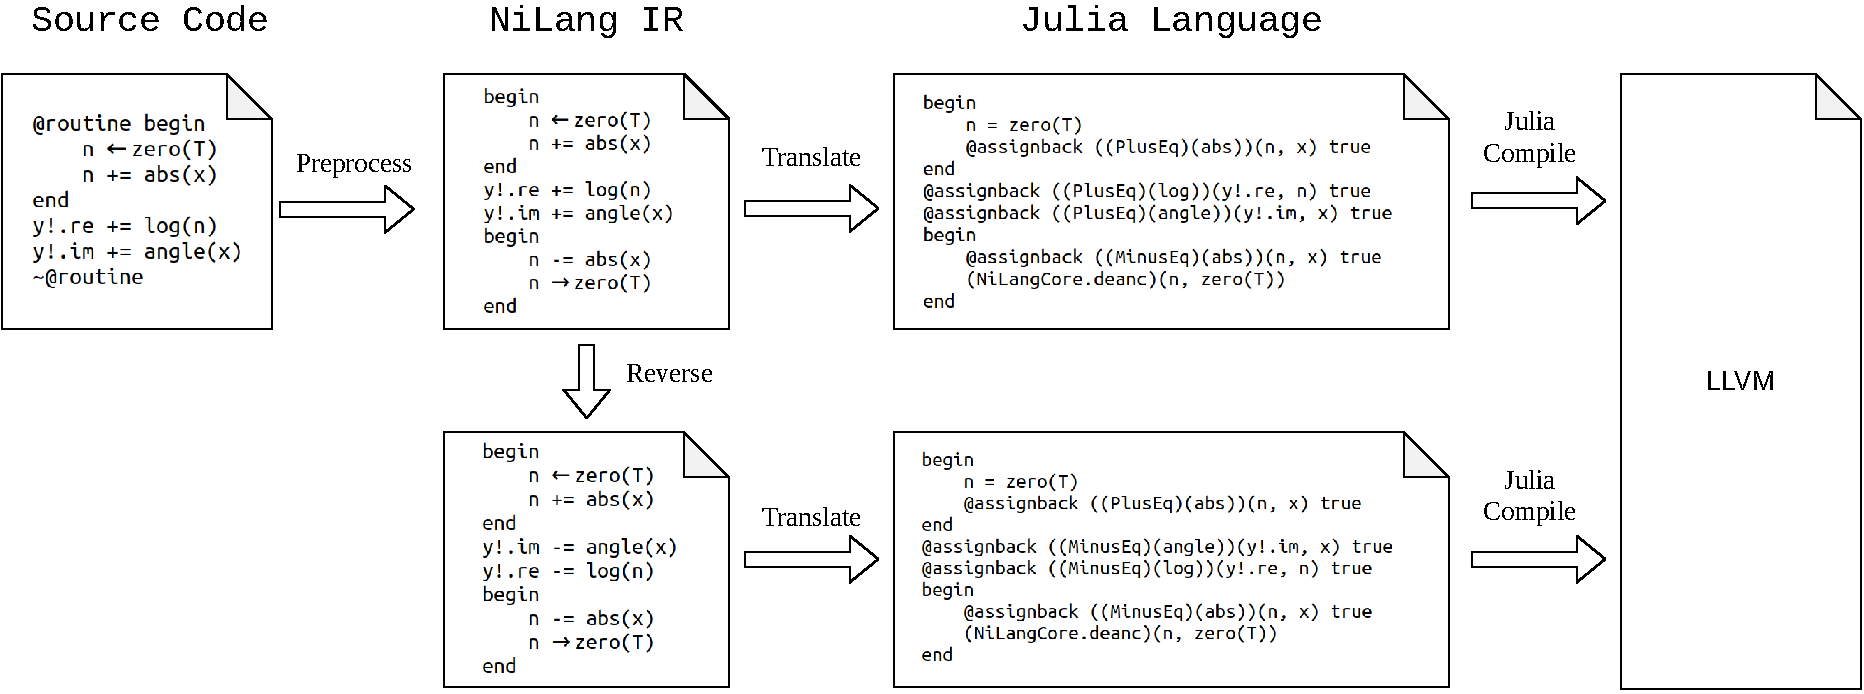
\includegraphics[width=0.95\columnwidth,trim={0cm 0cm 0cm 0cm},clip]{compiling_v2.pdf}}
    \caption{Compiling the body of the complex valued log function defined in \Lst{lst:complex}.}\label{fig:compiling}
\end{figure}

In the \textit{preprocessing} stage, the compiler pre-processes human inputs to the reversible NiLang IR.
The preprocessor removes redundant grammars and expands shortcuts. In the left most code box in \Fig{fig:compiling}, one uses \texttt{@routine <stmt>} statement to record a statement, and \texttt{$\sim$@routine} to insert the corresponding inverse statement for uncomputing.
The computing-uncomputing macros \texttt{@routine} and \texttt{$\sim$@routine} is expanded in this stage.
In the \textit{reversing} stage, based on this symmetric and reversible IR, the compiler generates reversed statements.
In the \textit{translation} stage, the compiler translates this reversible IR as well as its inverse to native Julia code. It adds \texttt{@assignback} before each function call, inserts codes for reversibility check, and handle control flows.
As a final step, the compiler attaches a return statement that returns all updated input arguments at the end of a function definition.
Now, the function is ready to execute on the host language.


\subsection{NiLang Grammar}\label{app:grammar}
To define a reversible function one can use ``@i'' plus a standard function definition like bellow

\begin{minipage}{.88\columnwidth}
\begin{lstlisting}[basicstyle=\small\ttfamily,columns=fullflexible]
"""
docstring...
"""
@i function f(args..., kwargs...) where {...}
    <stmts>
end
\end{lstlisting}
\end{minipage}
where the definition of ``<stmts>'' are shown in the grammar page bellow.
The following is a list of terminologies used in the definition of grammar
\begin{itemize}
    \item $ident$, symbols
    \item $num$, numbers
    \item $\epsilon$, empty statement
    \item $JuliaExpr$, native Julia expression
    \item $[$ $]$,  zero or one repetitions.
\end{itemize}
Here, all $JuliaExpr$ should be pure. Otherwise, the reversibility is not guaranteed.
Dataview is a view of data. It can be a bijective mapping of an object, an item of an array, or a field of an object.

\newpage

\begin{minipage}{0.6\textwidth}
    \small
\begin{bnf*}
    \bnfprod{Stmts}{\bnfsp \bnfes}\\
    \bnfmore{\bnfor \bnfpn{Stmt}}\\
    \bnfmore{\bnfor \bnfpn{Stmts} \bnfsp \bnfpn{Stmt}}\\
    \bnfprod{Stmt}{\bnfpn{BlockStmt}}\\
    \bnfmore{\bnfor \bnfpn{IfStmt}}\\
    \bnfmore{\bnfor \bnfpn{WhileStmt}}\\
    \bnfmore{\bnfor \bnfpn{ForStmt}}\\
    \bnfmore{\bnfor \bnfpn{InstrStmt}}\\
    \bnfmore{\bnfor \bnfpn{RevStmt}}\\
    \bnfmore{\bnfor \bnfpn{@anc} \bnfsp \bnfpn{Stmt}}\\
    \bnfmore{\bnfor \bnfpn{@routine} \bnfsp \bnfpn{Stmt}}\\
    \bnfmore{\bnfor \bnfpn{@safe} \bnfsp \bnftd{$JuliaExpr$}}\\
    \bnfmore{\bnfor \bnfpn{CallStmt}}\\
    \bnfprod{BlockStmt}{\bnftd{begin} \bnfsp \bnfpn{Stmts} \bnfsp \bnftd{end}}\\
    \bnfprod{RevCond}{\bnftd{(} \bnfsp \bnftd{$JuliaExpr$} \bnfsp \bnftd{,} \bnfsp \bnftd{$JuliaExpr$} \bnfsp \bnftd{)}}\\
    \bnfprod{IfStmt}{\bnftd{if} \bnfsp \bnfpn{RevCond} \bnfsp \bnfpn{Stmts} \bnfsp \bnfts{[} \bnftd{else} \bnfsp \bnfpn{Stmts}\bnfts{]} \bnfsp \bnftd{end}}\\
    \bnfprod{WhileStmt}{\bnftd{while} \bnfsp \bnfpn{RevCond} \bnfsp \bnfpn{Stmts} \bnfsp \bnftd{end}}\\
    \bnfprod{Range}{\bnftd{$JuliaExpr$} \bnfsp \bnftd{:} \bnfsp \bnftd{$JuliaExpr$} \bnfsp \bnfts{[} \bnftd{:} \bnfsp \bnftd{$JuliaExpr$}\bnfts{]}}\\
    \bnfprod{ForStmt}{\bnftd{for} \bnfsp \bnftd{ident} \bnfsp \bnftd{=} \bnfsp \bnfpn{Range} \bnfsp \bnfpn{Stmts} \bnfsp \bnftd{end}}\\
    \bnfprod{CallStmt}{\bnftd{$JuliaExpr$} \bnfsp \bnftd{(} \bnfsp \bnfts{[} \bnfpn{DataViews}\bnfts{]} \bnfsp \bnftd{)}}\\
    \bnfprod{Constant}{\bnftd{num} \bnfor \bnftd{$\pi$}}\\
    \bnfprod{InstrBinOp}{\bnftd{+=} \bnfor \bnftd{-=} \bnfor \bnftd{$\veebar$=}}\\
    \bnfprod{InstrTrailer}{\bnfts{[} \bnftd{.}\bnfts{]} \bnfsp \bnftd{(} \bnfsp \bnfts{[} \bnfpn{DataViews}\bnfts{]} \bnfsp \bnftd{)}}\\
    \bnfprod{InstrStmt}{\bnfpn{DataView} \bnfsp \bnfpn{InstrBinOp} \bnfsp \bnftd{ident} \bnfsp \bnfts{[} \bnfpn{InstrTrailer}\bnfts{]}}\\
    \bnfprod{RevStmt}{\bnftd{$\sim$} \bnfsp \bnfpn{Stmt}}\\
    \bnfprod{@routine}{\bnftd{@routine} \bnfsp \bnftd{ident} \bnfsp \bnfpn{Stmt}}\\
    \bnfprod{AncArg}{\bnftd{ident} \bnfsp \bnftd{=} \bnfsp \bnftd{$JuliaExpr$}}\\
    \bnfprod{@anc}{\bnftd{@anc} \bnfsp \bnfpn{AncArg}}\\
    \bnfmore{\bnfor \bnftd{@deanc} \bnfsp \bnfpn{AncArg}}\\
    \bnfprod{@safe}{\bnftd{@safe} \bnfsp \bnftd{$JuliaExpr$}}\\
    \bnfprod{DataViews}{\bnfsp \bnfes}\\
    \bnfmore{\bnfor \bnfpn{DataView}}\\
    \bnfmore{\bnfor \bnfpn{DataViews} \bnfsp \bnftd{,} \bnfsp \bnfpn{DataView}}\\
    \bnfprod{DataView}{\bnfpn{DataView} \bnfsp \bnftd{[} \bnfsp \bnftd{$JuliaExpr$} \bnfsp \bnftd{]}}\\
    \bnfmore{\bnfor \bnfpn{DataView} \bnfsp \bnftd{.} \bnfsp \bnftd{ident}}\\
    \bnfmore{\bnfor \bnftd{$JuliaExpr$} \bnfsp \bnftd{(} \bnfsp \bnfpn{DataView} \bnfsp \bnftd{)}}\\
    \bnfmore{\bnfor \bnfpn{Constant}}\\
    \bnfmore{\bnfor \bnftd{ident}}\\
\end{bnf*}

\end{minipage}

\Tbl{tbl:revstatements} shows the meaning of some selected statements and how they are reversed.

\begin{table}[h!]\centering
    \footnotesize
\begin{minipage}{\columnwidth}
\ra{1.3}
    \scalebox{1.0}{
        \begin{tabularx}{\textwidth}{X X X}\toprule
            \textbf{Statement} & \textbf{Meaning} & \textbf{Inverse}\\
            \hline
            \texttt{<f>(<args>...)} & function call & \texttt{($\sim$<f>)(<args>...)}\\
            \hline
            \texttt{<f>.(<args>...)} & broadcast a function call & \texttt{<f>.(<args>...)}\\
            \hline
            \texttt{<y> += <f>(<args>...)} & inplace add instruction & \texttt{<y> -= <f>(<args>...)}\\
            \hline
            \texttt{<y> $\veebar$= <f>(<args>...)} & inplace XOR instruction & \texttt{<y> $\veebar$= <f>(<args>...)}\\
            \hline
            \texttt{<a> $\leftarrow$ <expr>} & allocate a new variable & \texttt{<a> $\rightarrow$ <expr>}\\
            \hline
            \texttt{begin}\newline \texttt{$\cquad$<stmts>}\newline \texttt{end} & statement block & \texttt{begin}\newline \texttt{$\cquad$ $\sim$(<stmts>)}\newline \texttt{end}\\
            \hline
            \texttt{if (<pre>, <post>)}\linebreak \texttt{$\cquad$<stmts1>}\newline \texttt{else}\newline \texttt{$\cquad$<stmts2>}\newline \texttt{end} & if statement & \texttt{if (<post>, <pre>)}\newline \texttt{$\cquad$$\sim$(<stmts1>)}\newline \texttt{else}\newline \texttt{$\cquad$ $\sim$(<stmts2>)}\newline \texttt{end}\\ %$
            \hline
            \texttt{while (<pre>, <post>)}\newline \texttt{$\cquad$<stmts>} \newline \texttt{end} & while statement & \texttt{while (<post>, <pre>)}\newline $\cquad$  \texttt{$\sim$(<stmts>)}\newline \texttt{end}\\
            \hline
            \texttt{for <i>=<m>:<s>:<n>}\newline $\cquad$\texttt{<stmts>}\newline \texttt{end} & for statement & \texttt{for <i>=<m>:-<s>:<n>}\newline $\cquad$ \texttt{$\sim$(<stmts>)}\newline \texttt{end}\\
            \bottomrule
        \end{tabularx}
    }
    \caption{Basic statements in NiLang IR.
    ``$\sim$'' is the symbol for reversing a statement or a function.
    ``.'' is the symbol for the broadcasting magic in Julia,
    \texttt{<pre>} stands for precondition, and \texttt{<post>} stands for postcondition
``\texttt{begin <stmts> end}'' is the code block statement in Julia.
It can be inverted by reversing the order as well as each element in it.
}\label{tbl:revstatements}
\end{minipage}
\end{table}

\newpage
\subsection{Instructions Used in Main Text}\label{app:instr}

A table instructions used in the main text
\begin{table}[h!]\centering
\begin{minipage}{0.8\columnwidth}
\ra{1.3}
    \scalebox{1.0}{
        \begin{tabularx}{\textwidth}{X X}\toprule
            \textbf{instruction} & \textbf{output}\\
            \hline
            ${\rm SWAP}(a, b)$ & $b, a$\\
            ${\rm ROT}(a, b, \theta)$ & $a \cos\theta - b\sin\theta, b \cos\theta + a\sin\theta, \theta$\\
            ${\rm IROT}(a, b, \theta)$ & $a \cos\theta + b\sin\theta, b \cos\theta - a\sin\theta, \theta$\\
            $y \pluseq a * b$ & $y+a*b, a, b$\\
            $y \pluseq a / b$ & $y+a/b, a, b$\\
            $y \pluseq a^\wedge b$ & $y+a^b, a, b$\\
            $y \pluseq {\rm identity}(x)$ & $y+x, x$\\
            $y \pluseq \exp(x)$ & $y+e^x, x$\\
            $y \pluseq \log(x)$ & $y+\log x, x$\\
            $y \pluseq \sin(x)$ & $y+\sin x, x$\\
            $y \pluseq \cos(x)$ & $y+\cos x, x$\\
            $y \pluseq {\rm abs}(x)$ & $y+ |x|, x$\\
            ${\rm NEG}(y)$ & $-y$\\
            ${\rm INC}(y)$ & $y+1$\\
            ${\rm DEC}(y)$ & $y-1$\\
            \bottomrule
        \end{tabularx}
    }
    \caption{Predefined reversible instructions in NiLang.}\label{tbl:revinstructions}
\end{minipage}
\end{table}

\subsection{Reversible Constructors}\label{app:constructor}
So far, the language design is not too different from a traditional reversible language. To port Julia's type system better, we introduce dataviews.
The type used in the reversible context is just a standard Julia type with an additional requirement of having reversible constructors.
The inverse of a constructor is called a ``destructor'', which unpacks data and deallocates derived fields.
A reversible constructor is implemented by reinterpreting the \texttt{new} function in Julia.
Let us consider the following statement.

\begin{minipage}{.88\columnwidth}
\begin{lstlisting}
    x ← new{TX, TG}(x, g)
\end{lstlisting}
\end{minipage}

The above statement is similar to allocating an ancilla, except that it deallocates \texttt{g} directly at the same time.
Doing this is proper because \texttt{new} is special that its output keeps all information of its arguments. All input variables that do not appear in the output can be discarded safely. Its inverse is

\begin{minipage}{.88\columnwidth}
\begin{lstlisting}
    x → new{TX, TG}(x, g)
\end{lstlisting}
\end{minipage}

It unpacks structure \texttt{x} and assigns fields to corresponding variables in the argument list.
The following example shows a non-complete definition of the reversible type \texttt{GVar}.

\begin{minipage}{\columnwidth}
\begin{lstlisting}[multicols=2]
julia> using NiLangCore

julia> @i struct GVar{T,GT} <: IWrapper{T}
           x::T
           g::GT
           function GVar{T,GT}(x::T, g::GT)
                        where {T,GT}
               new{T,GT}(x, g)
           end
           function GVar(x::T, g::GT)
                        where {T,GT}
               new{T,GT}(x, g)
           end
           @i function GVar(x::T) where T
               g ← zero(x)
               x ← new{T,T}(x, g)
           end
           @i function GVar(x::AbstractArray)
               GVar.(x)
           end
       end

julia> GVar(0.5)
GVar{Float64,Float64}(0.5, 0.0)

julia> (~GVar)(GVar(0.5))
0.5

julia> (~GVar)(GVar([0.5, 0.6]))
2-element Array{Float64,1}:
 0.5
 0.6
\end{lstlisting}
\end{minipage}

\texttt{GVar} has two fields that correspond to the value and gradient of a variable.
Here, we put \texttt{@i} macro before both \texttt{struct} and \texttt{function} statements.
The ones before functions generate forward and backward functions, while the one before \texttt{struct} moves \texttt{$\sim$GVar} functions to the outside of the type definition. Otherwise, the inverse function will be ignored by Julia compiler.

Since an operation changes data inplace in NiLang, a field of an immutable instance should also be `` modifiable''.
Let us first consider the following example.

\begin{minipage}{.88\columnwidth}
\begin{lstlisting}
julia> arr = [GVar(3.0), GVar(1.0)]
2-element Array{GVar{Float64,Float64},1}:
 GVar{Float64,Float64}(3.0, 0.0)
 GVar{Float64,Float64}(1.0, 0.0)

julia> x, y = 1.0, 2.0
(1.0, 2.0)

julia> @instr -arr[2].g += x * y
2.0

julia> arr
2-element Array{GVar{Float64,Float64},1}:
 GVar{Float64,Float64}(3.0, 0.0) 
 GVar{Float64,Float64}(1.0, -2.0)
\end{lstlisting}
\end{minipage}

In Julia language, the assign statement above will throw a syntax error because the function call ``\texttt{-}'' can not be assigned, and \texttt{GVar} is an immutable type.
In NiLang, we use the macro \texttt{@assignback} to modify an immutable data directly. It translates the above statement to

\begin{minipage}{.88\columnwidth}
\begin{lstlisting}[numberstyle=\scriptsize\color{gray},numbers=left,numbersep=8pt]
res = (PlusEq(*))(-arr[2].g, x, y)
arr[2] = chfield(arr[2], Val(:g),
    chfield(arr[2].g, -, res[1]))
x = res[2]
y = res[3]
\end{lstlisting}
\end{minipage}

The first line \texttt{PlusEq(*)(-arr[3].g, x, y)} computes the output as a tuple of length $3$.
At lines 2-3, \texttt{chfield(x, Val\{:g\}, val)} modifies the \texttt{g} field of \texttt{x} and \texttt{chfield(x, -, res[1])} returns \texttt{-res[1]}. Here, modifying a field requires the default constructor of a type not overwritten.
The assignments in lines 4 and 5 are straightforward.
We call a bijection of a field of an object a ``dataview'' of this object, and it is directly modifiable in NiLang.
The definition of dataview can be found in \App{app:grammar}.

\section{Examples}\label{sec:example}

In this section, we introduce several examples.
\begin{list}{$\circ$}{}
\item sparse matrix dot product,
\item first kind bessel function and memory oriented computational graph,
\item solving the graph embedding problem.
\end{list}

All codes for this section and the next benchmark section are available in the \href{https://github.com/GiggleLiu/nilangpaper}{paper repository}.

\subsection{Sparse Matrices}
Differentiating sparse matrices is useful in many applications, however, it can not benefit directly from generic backward rules for the dense matrix because the generic rules do not keep the sparse structure.
In the following, we will show how to convert a irreversible Frobenius dot product code to a reversible one to differentiate it.
Here, the Frobenius dot product is defined as \texttt{trace(A\textquotesingle B)}.
In SparseArrays code base, it is implemented as follows.

\begin{minipage}{\columnwidth}
\begin{lstlisting}[multicols=2]
function dot(A::AbstractSparseMatrixCSC{T1,S1}, B::AbstractSparseMatrixCSC{T2,S2}
      ) where {T1,T2,S1,S2}
  m, n = size(A)
  size(B) == (m,n) || throw(DimensionMismatch("matrices must have the same dimensions"))
  r = dot(zero(T1), zero(T2))
  @inbounds for j = 1:n
    ia = getcolptr(A)[j]
    ia_nxt = getcolptr(A)[j+1]
    ib = getcolptr(B)[j]
    ib_nxt = getcolptr(B)[j+1]
    if ia < ia_nxt && ib < ib_nxt
      ra = rowvals(A)[ia]
      rb = rowvals(B)[ib]
      while true
        if ra < rb
          ia += oneunit(S1)
          ia < ia_nxt || break
          ra = rowvals(A)[ia]
        elseif ra > rb
          ib += oneunit(S2)
          ib < ib_nxt || break
          rb = rowvals(B)[ib]
        else # ra == rb
          r += dot(nonzeros(A)[ia],
                nonzeros(B)[ib])
          ia += oneunit(S1)
          ib += oneunit(S2)
          ia < ia_nxt && ib < ib_nxt || break
          ra = rowvals(A)[ia]
          rb = rowvals(B)[ib]
        end
      end
    end
  end
  return r
end
\end{lstlisting}
\end{minipage}


It is easy to rewrite it in a reversible style with NiLang without sacrificing much performance.

\begin{minipage}{\columnwidth}
\begin{lstlisting}[multicols=2]
@i function dot(r::T, A::SparseMatrixCSC{T}, B::SparseMatrixCSC{T}) where {T}
    m ← size(A, 1)
    n ← size(A, 2)
    @invcheckoff branch_keeper ← zeros(Bool,2*m)
    @safe size(B) == (m,n) || throw(DimensionMismatch("matrices must have the same dimensions"))
    @invcheckoff @inbounds for j = 1:n
        ia1 ← A.colptr[j]
        ib1 ← B.colptr[j]
        ia2 ← A.colptr[j+1]
        ib2 ← B.colptr[j+1]
        ia ← ia1
        ib ← ib1
        @inbounds for i=1:ia2-ia1+ib2-ib1-1
            ra ← A.rowval[ia]
            rb ← B.rowval[ib]
            if (ra == rb, ~)
                r += A.nzval[ia]'*B.nzval[ib]
            end
            # b move -> true, a move -> false
            branch_keeper[i] ⊻= ia==ia2-1 ||
                ra > rb
            ra → A.rowval[ia]
            rb → B.rowval[ib]
            if (branch_keeper[i], ~)
                ib += identity(1)
            else
                ia += identity(1)
            end
        end

        ~@inbounds for i=1:ia2-ia1+ib2-ib1-1
            # b move -> true, a move -> false
            branch_keeper[i] ⊻= ia==ia2-1 ||
                A.rowval[ia] > B.rowval[ib]
            if (branch_keeper[i], ~)
                ib += identity(1)
            else
                ia += identity(1)
            end
        end
    end
    @invcheckoff branch_keeper → zeros(Bool, 2*m)
end
\end{lstlisting}
\end{minipage}

Here, all assignments are replaced with \texttt{$\leftarrow$} to indicate that the values of these variables must be returned at the end of this function scope.
We put a ``\texttt{$\sim$}'' symbol in the postcondition field of if statements to indicate this postcondition is a dummy one that takes the same value as the precondition, i.e. the condition is not changed inside the loop body.
If the precondition is changed by the loop body, one can use a \texttt{branch\_keeper} vector to cache branch decisions. The value of \texttt{branch\_keeper} can be restored through uncomputing (the ``$\sim$'' statement above).
Finally, after checking the correctness of the program, one can turn off the reversibility checks by using the macro \texttt{@invcheckoff} macro to achieve better performance.

\subsection{The first kind Bessel function}\label{sec:bessel}
A Bessel function of the first kind of order $\nu$ can be computed via Taylor expansion
\begin{equation}
    J_\nu(z) = \sum\limits_{n=0}^{\infty} \frac{(z/2)^\nu}{\Gamma(\nu+1)\Gamma(k+\nu+1)} (-z^2/4)^{n}
\end{equation}
where $\Gamma(n) = (n-1)!$ is the Gamma function. One can compute the accumulated item iteratively as $s_n = -\frac{z^2}{4} s_{n-1}$. The irreversible implementation is

\begin{minipage}{.88\columnwidth}
\begin{lstlisting}
function besselj(ν, z; atol=1e-8)
    k = 0
    s = (z/2)^ν / factorial(ν)
    out = s
    while abs(s) > atol
        k += 1
        s *= (-1) / k / (k+ν) * (z/2)^2
        out += s
    end
    out
end
\end{lstlisting}
\end{minipage}

This computational process could be diagrammatically represented as a computational graph as shown in \Fig{fig:cgraphs} (a).
The computational graph is a directed acyclic graph (DAG), where a node is a function and an edge is a data.
An edge connects two nodes, one generates this data, and one consumes it.
A computational graph is more likely a mathematical expression. It can not describe inplace functions and control flows conveniently because it does not have the notation for memory and loops.
\begin{figure*}[t!]
    \centering
    \begin{subfigure}[t]{0.52\textwidth}
        \centering
        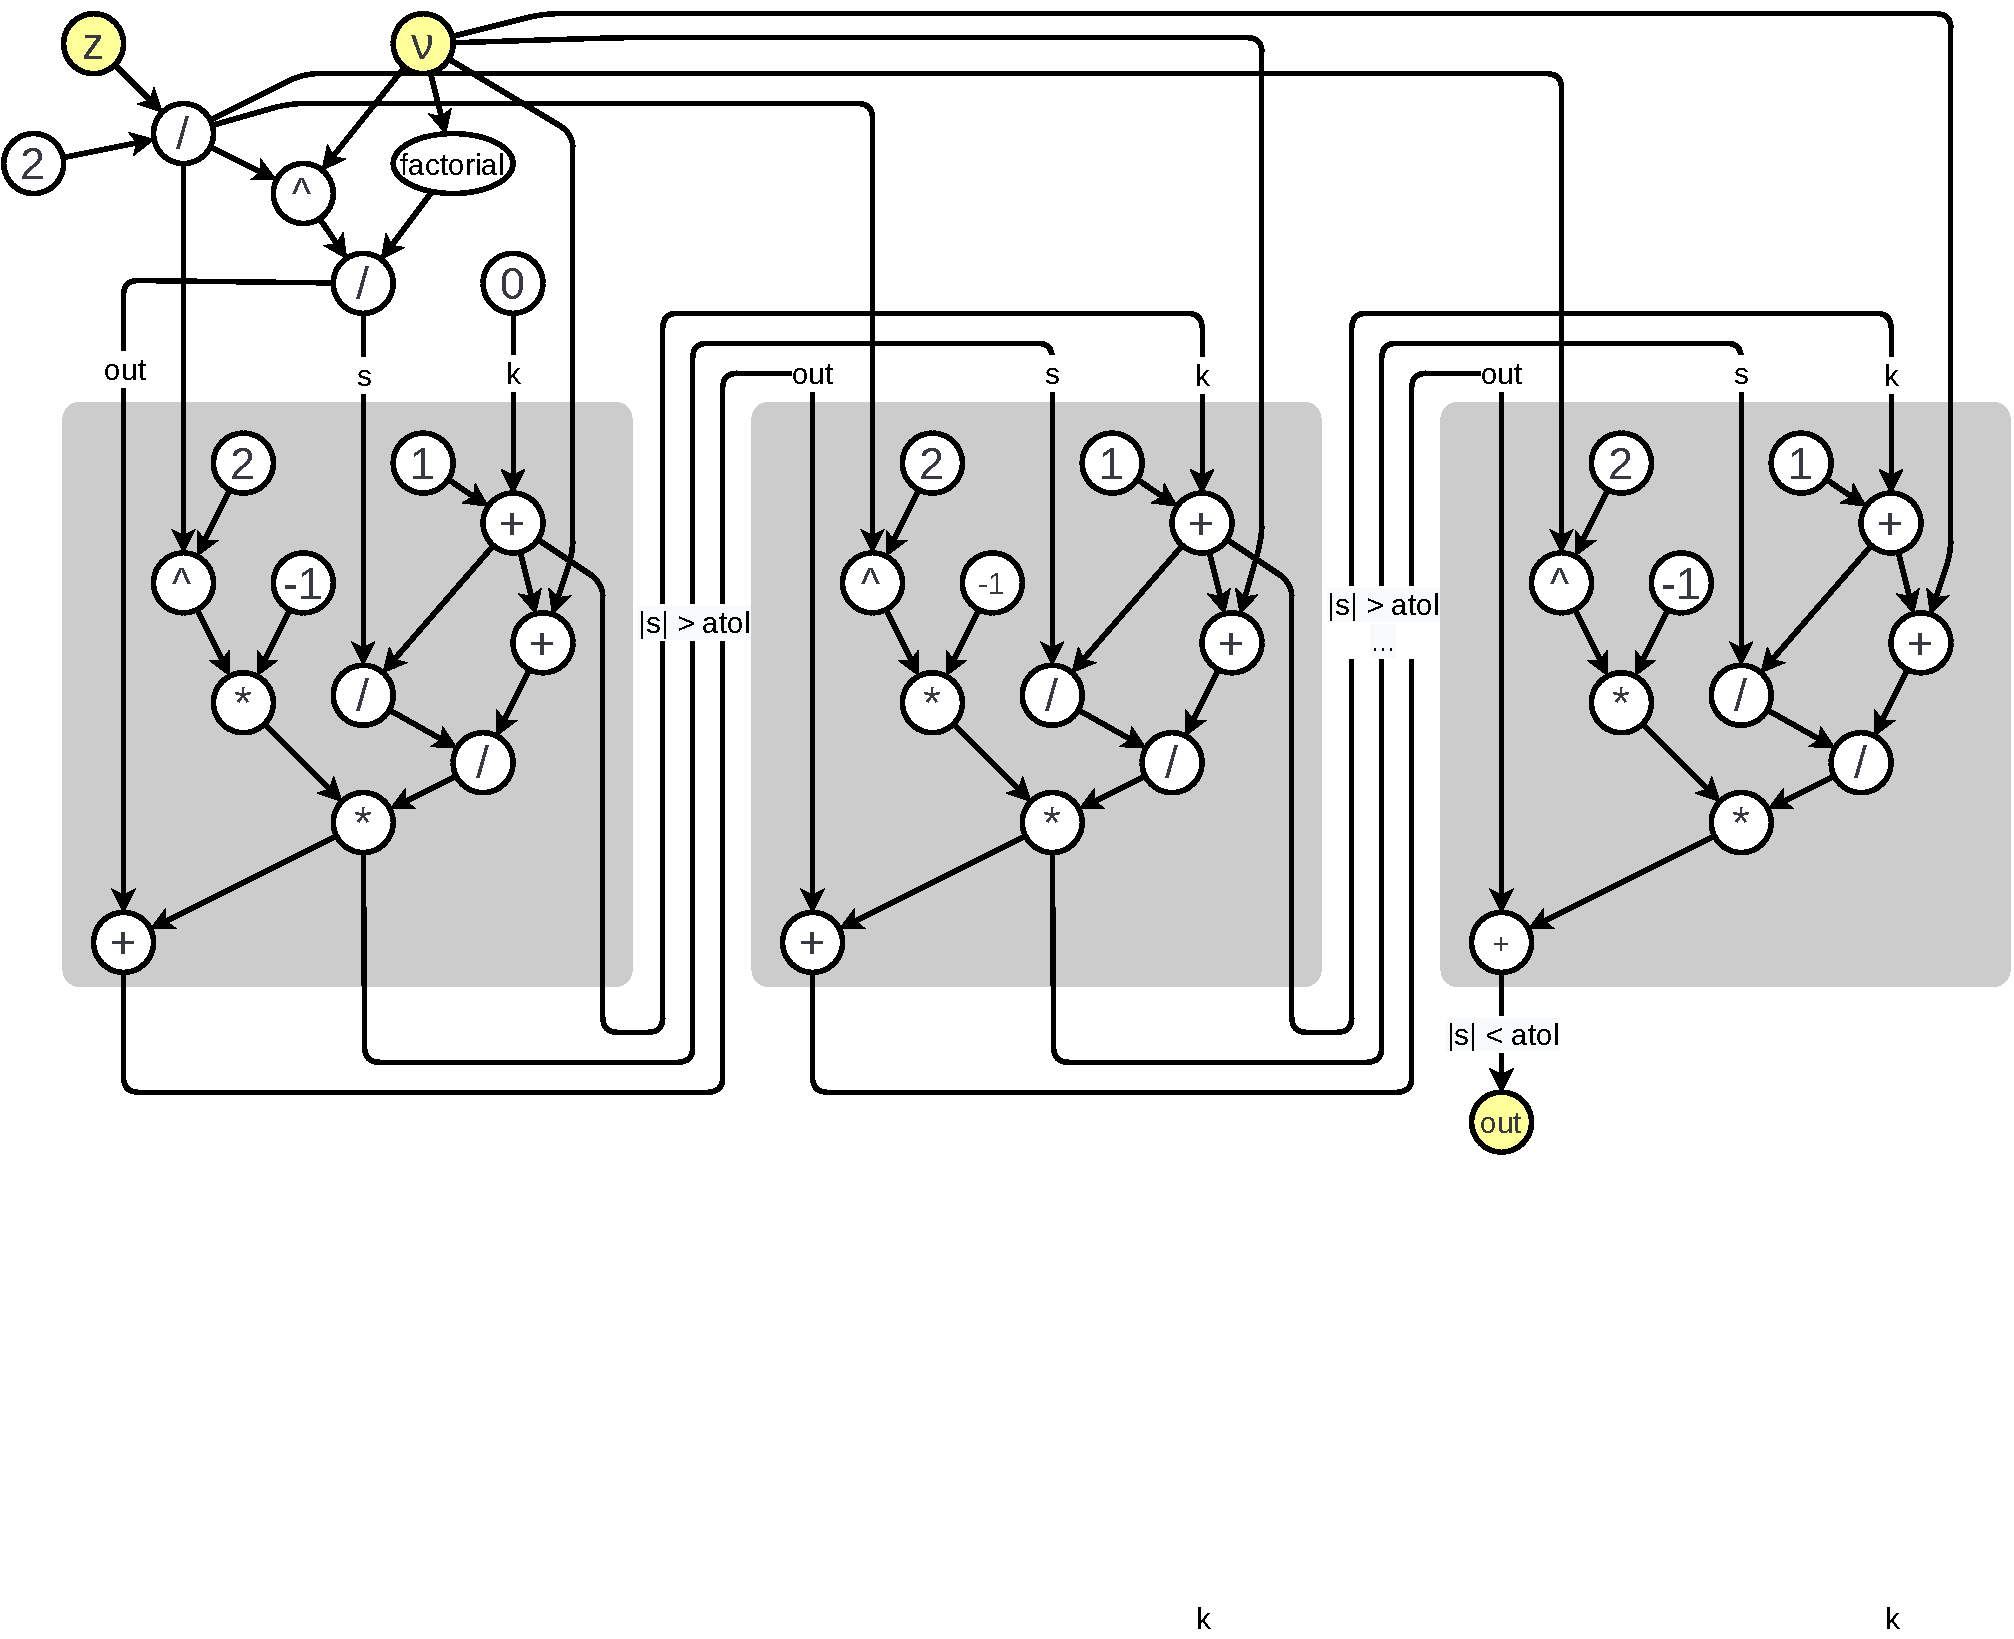
\includegraphics[width=\textwidth,trim={0 4cm 0 0cm},clip]{computational_graph.pdf}
        \caption{}
    \end{subfigure}%
    ~
    \begin{subfigure}[t]{0.47\textwidth}
        \centering
        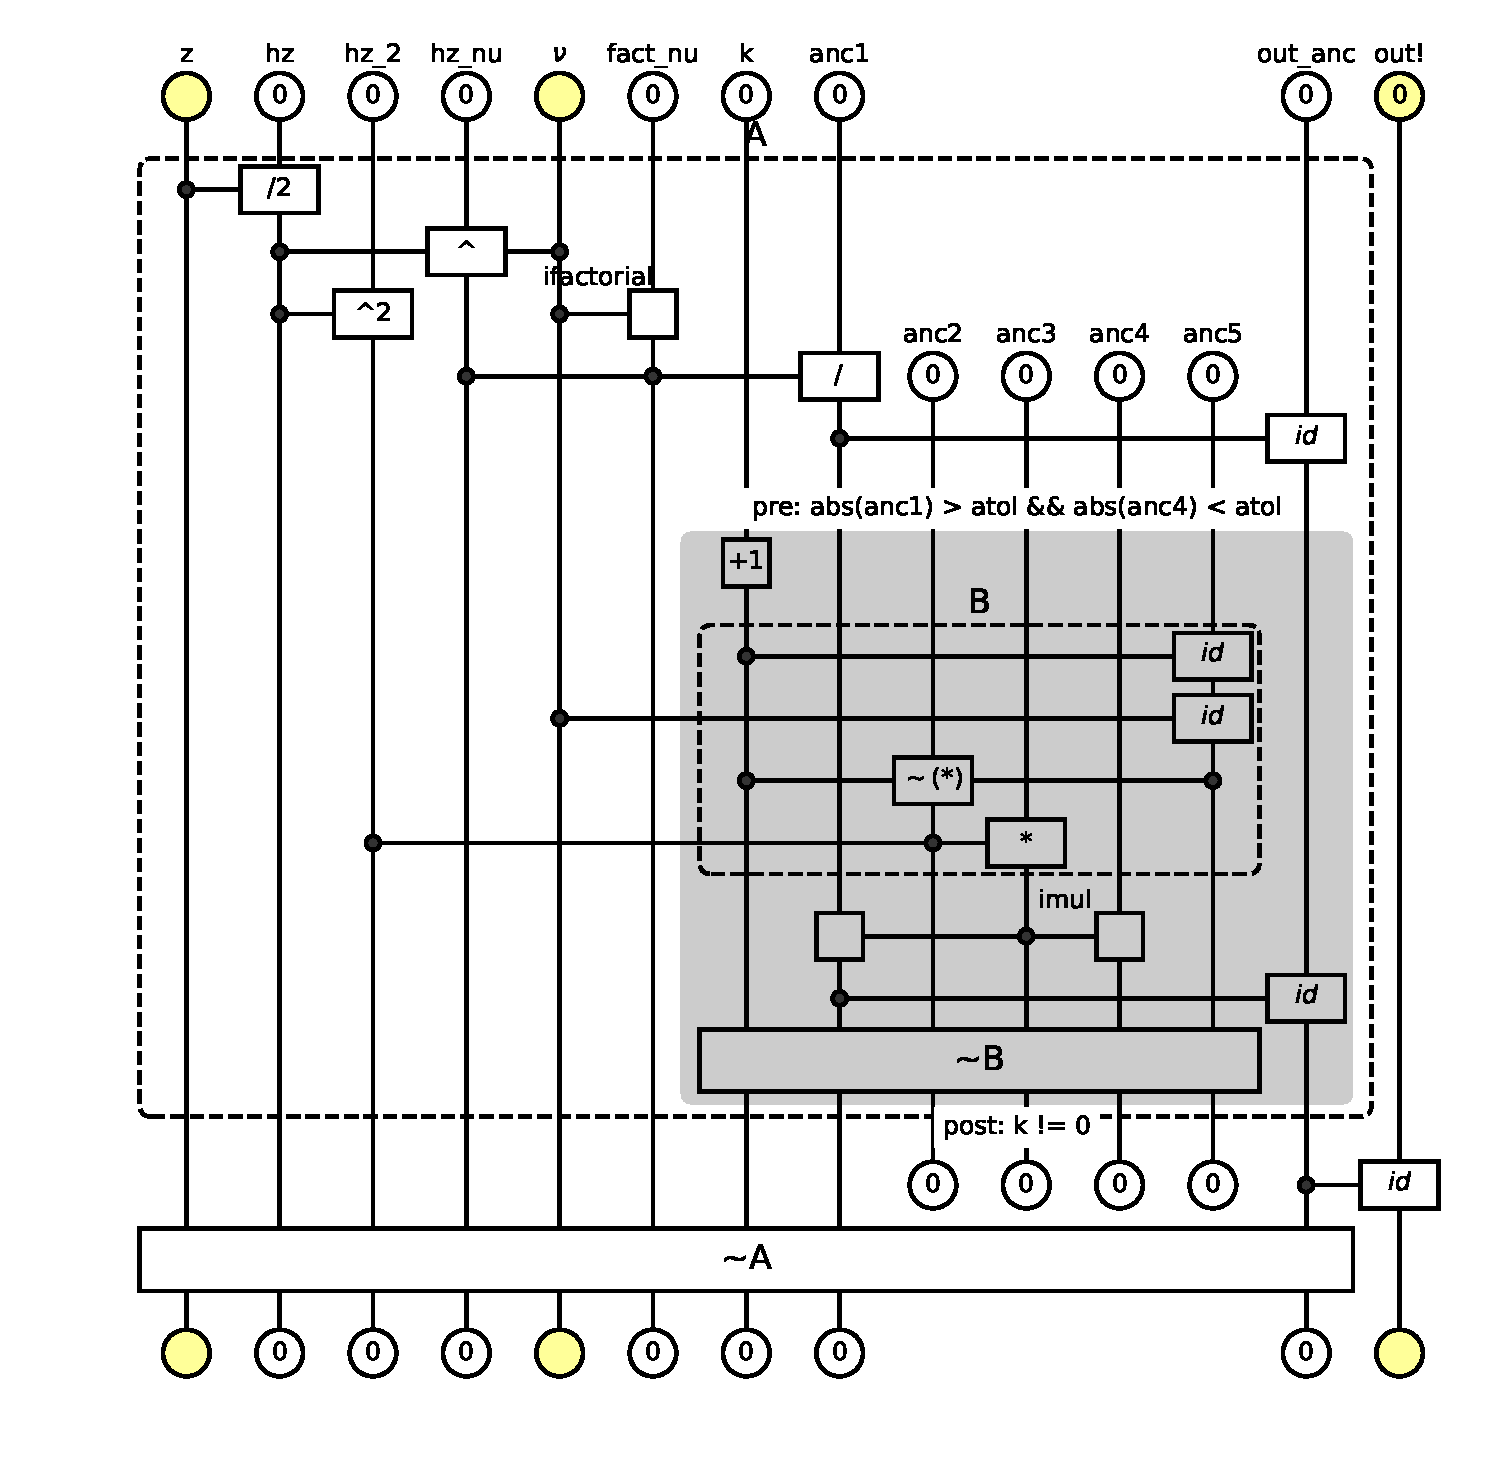
\includegraphics[width=\textwidth,trim={0 1cm 0 0cm},clip]{fig4.pdf}
        \caption{}
    \end{subfigure}
    \caption{(a) The traditional computational graph for the irreversible implementation of the first kind Bessel function. A vertex (circle) is an operation, and a directed edge is a variable. The gray regions are the body of the unrolled while loop.
        (b) The memory oriented computational graph for the reversible implementation of the first kind Bessel function. Notations are explained in \Fig{fig:ccu}.
    The gray region is the body of a while loop. Its precondition and postcondition are positioned on the top and bottom, respectively.
    }\label{fig:cgraphs}
\end{figure*}

With the logarithmic number system, we implement the reversible $J_\nu$ as follows.

\begin{minipage}{\columnwidth}
\begin{lstlisting}[multicols=2]
@i function ibesselj(y!::T, ν, z::T; atol=1e-8) where T
	if z == 0
		if v == 0
			out! += 1
		end
	else
		@routine @invcheckoff begin
			k ← 0
			@ones ULogarithmic{T} lz halfz halfz_power_2 s
			@zeros T out_anc
			lz *= convert(z)
			halfz *= lz / 2
			halfz_power_2 *= halfz ^ 2
			# s *= (z/2)^ν/ factorial(ν)
			s *= halfz ^ ν
			for i=1:ν
				s /= i
			end
			out_anc += convert(s)
			while (s.log > -25, k!=0) # upto precision e^-25
				k += 1
				# s *= 1 / k / (k+ν) * (z/2)^2
				s *= halfz_power_2 / (k*(k+ν))
				if k%2 == 0
					out_anc += convert(s)
				else
					out_anc -= convert(s)
				end
			end
		end
		y! += out_anc
		~@routine
	end
end
\end{lstlisting}
\end{minipage}

The above algorithm uses a constant number of ancillas, while the time overhead is also a constant.
This reversible program can be diagrammatically represented as a memory oriented computational graph as shown in \Fig{fig:cgraphs} (b).
This diagram can be used to analyze variables uncomputing.
%So far, the coversion between logarithmic system and fixed/floating point number system are not efficiently implemented.

One can obtain gradients of this function by calling \texttt{Grad(ibesselj)}.
\begin{minipage}{.88\columnwidth}
\begin{lstlisting}
julia> out!, x = 0.0, 1.0
(0.0, 1.0)

julia> Grad(ibesselj)(Val(1), out!, 2, x)
(Val{1}(), GVar(0.0, 1.0), 2, GVar(1.0, 0.2102436))
\end{lstlisting}
\end{minipage}

Here, \texttt{Grad(ibesselj)} returns a callable instance of type \texttt{Grad\{typeof(ibesselj)\}}. The first parameters \texttt{Val(1)} specifies the position of loss in argument list. 
The Hessian can be obtained by feeding dual-numbers into this gradient function.

\begin{minipage}{.88\columnwidth}
\begin{lstlisting}
julia> out!, x = 0.0, 1.0
(0.0, 1.0)

julia> Grad(ibesselj)(Val(1), out!, 2, x)
(Val{1}(), GVar(0.0, 1.0), 2, GVar(1.0, 0.2102436))

julia> using ForwardDiff: Dual

julia> _, hxout!, _, hxx = Grad(ibesselj)(Val(1), 
        Dual(out!, zero(out!)), 2, Dual(x, one(x)));

julia> grad(hxx).partials[1]
0.13446683844358093
\end{lstlisting}
\end{minipage}

Here, the gradient field of \texttt{hxx} is defined as $\frac{\partial {\rm out!}}{\partial x}$, which is a Dual number.
It has a field \texttt{partials} that store the Hessian $\frac{\partial{\rm out!}^2}{\partial x^2}$.

\subsection{Solving a graph embedding problem}\label{sec:graph}
Graph embedding can be used to find a proper representation for an order parameter~\cite{Takahashi2020} in condensed matter physics.
\Ref{Takahashi2020} considers a problem of finding the minimum Euclidean space dimension $k$ that a Petersen graph can embed into, that the distances between pairs of connected vertices are $l_1$, and the distance between pairs of disconnected vertices are $l_2$, where $l_2 > l_1$.
The Petersen graph is shown in \Fig{fig:petersen}.
Let us denote the set of connected and disconnected vertex pairs as $L_1$ and $L_2$, respectively. This problem can be variationally solved with the following loss.
\begin{align}
    \begin{split}
        \mathcal{L} &= \Var({\rm dist}(L_1)) + \Var({\rm dist}(L_2)) \\
        &+\exp({\rm relu}(\overline{{\rm dist}(L_1)} - \overline{{\rm dist}(L_2)} + 0.1))) - 1
    \end{split}
\end{align}
The first line is a summation of distance variances in two sets of vertex pairs, where $\Var(X)$ is the variance of samples in $X$.
The second line is used to guarantee $l_2 > l_1$, where $\overline{X}$ means taking the average of samples in $X$.
Its reversible implementation could be found in our benchmark repository.

We repeat the training for dimension $k$ from $1$ to $10$.
In each training, we fix two of the vertices and optimize the positions of the rest. Otherwise, the program will find the trivial solution with overlapped vertices. 
For $k < 5$, the loss is always much higher than $0$,
while for $k\geq5$, we can get a loss close to machine precision with high probability.
From the $k=5$ solution, it is easy to see $l_2/l_1 = \sqrt{2}$.
An Adam optimizer with a learning rate $0.01$~\cite{Kingma2014} requires $\sim2000$ steps training.
The trust region Newton's method converges much faster, which requires $\sim 20$ computations of Hessians to reach convergence.
Although training time is comparable, the converged precision of the later is much better.
\begin{figure}
    \centerline{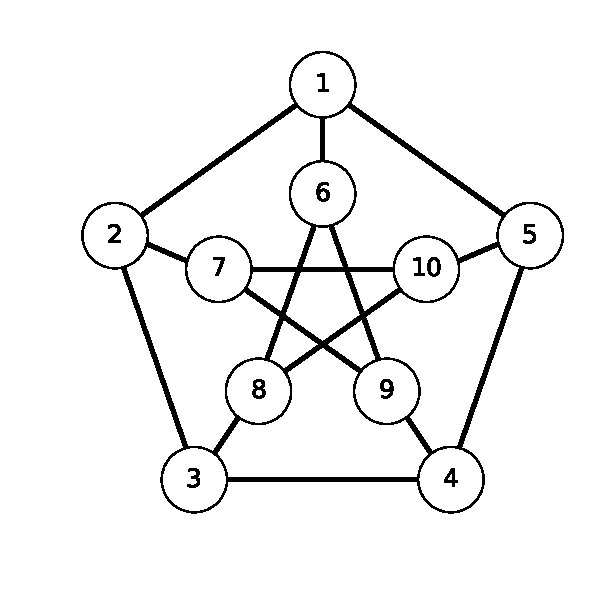
\includegraphics[width=0.4\columnwidth,trim={0 1cm 0 0},clip]{petersen.pdf}}
    \caption{The Petersen graph has 10 vertices and 15 edges. We want to find a minimum embedding dimension for it.}\label{fig:petersen}
\end{figure}


\subsection{Gaussian mixture model and bundle adjustment}
You will find the source code in github repositories \href{https://github.com/JuliaReverse/NiGaussianMixture.jl}{https://github.com/JuliaReverse/NiGaussianMixture.jl} and \href{https://github.com/JuliaReverse/NiBundleAdjustment.jl}{https://github.com/JuliaReverse/NiBundleAdjustment.jl}.

\section{Discussion and outlooks}\label{sec:discussion}
%In a reversible programming language, we proposed to use ``approximate uncomputing'' trick to avoid the overhead of a reversible program in many practical cases.
In this main text, we show how to realize a reversible programming eDSL and implement an instruction level backward mode AD on top of it.
It gives the user more flexibility to tradeoff memory and computing time comparing with traditional checkpointing.
The Julia implementation NiLang gives the state-of-the-art performance and memory efficiency in obtaining first and second-order gradients in applications, including first type Bessel function, sparse matrix manipulations, solving graph embedding problem, Gaussian mixture model and bundle adjustment. It provides the possibility to differentiate GPU kernels.
In the following, we discuss some practical issues about reversible programming, and several future directions to go.
%Notablely, we introduce the concept of ``arithematic uncomputing'' to reduce the overhead of recursive reversible algorithms.

\subsection{Time Space Tradeoff}\label{sec:timespace}
In history, there have been many discussions about time-space tradeoff on a reversible Turing machine (RTM).
In the most straightforward g-segment tradeoff scheme~\cite{Bennett1989,Levine1990}, an RTM model has either a space overhead that is proportional to computing time $T$ or a computational overhead that sometimes can be exponential to the program size comparing with an irreversible counterpart.
This result stops many people from taking reversible computing seriously as a high-performance computing scheme.
In the following, we try to explain why the overhead of reversible computing is not as terrible as people thought.

First of all, the overhead of reversing a program is upper bounded by the checkpointing~\cite{Chen2016} strategy used in many traditional machine learning package that memorizes inputs of primitives because checkpointing can be trivially implemented in reversible programming.~\cite{Perumalla2013} 
Reversible programming provides some alternatives to reduce the overhead.
For example, accumulation is reversible, so that many BLAS functions can be implemented reversiblly without extra memory.
Meanwhile, the memory allocation in some iterative algorithms can often be reduced by combining fixed point number and logarithmic numbers without sacrificing reversibility, as shown in the \texttt{ibesselj} example in \App{sec:bessel}.
Clever compiling based on memory oriented computational graphs (\Fig{fig:ccu} and \Fig{fig:cgraphs} (b)) can also be used to help user tradeoff between time and space.
The overhead of a reversible program mainly comes from the uncomputing of ancillas.
It is possible to automatically uncompute ancillas by analyzing variable dependency instead of asking users to write \texttt{@routine} and \texttt{$\sim$@routine} pairs.
In a hierarchical design, uncomputing can appear in every memory deallocation (or symbol table reduction). To quantify the overhead of uncomputing, we introduce the term uncomputing level as bellow.
\begin{definition}[uncomputing level]
    The log-ratio between the number of instructions of a reversible program and its irreversible counterpart.
\end{definition}

\begin{figure}
    \centerline{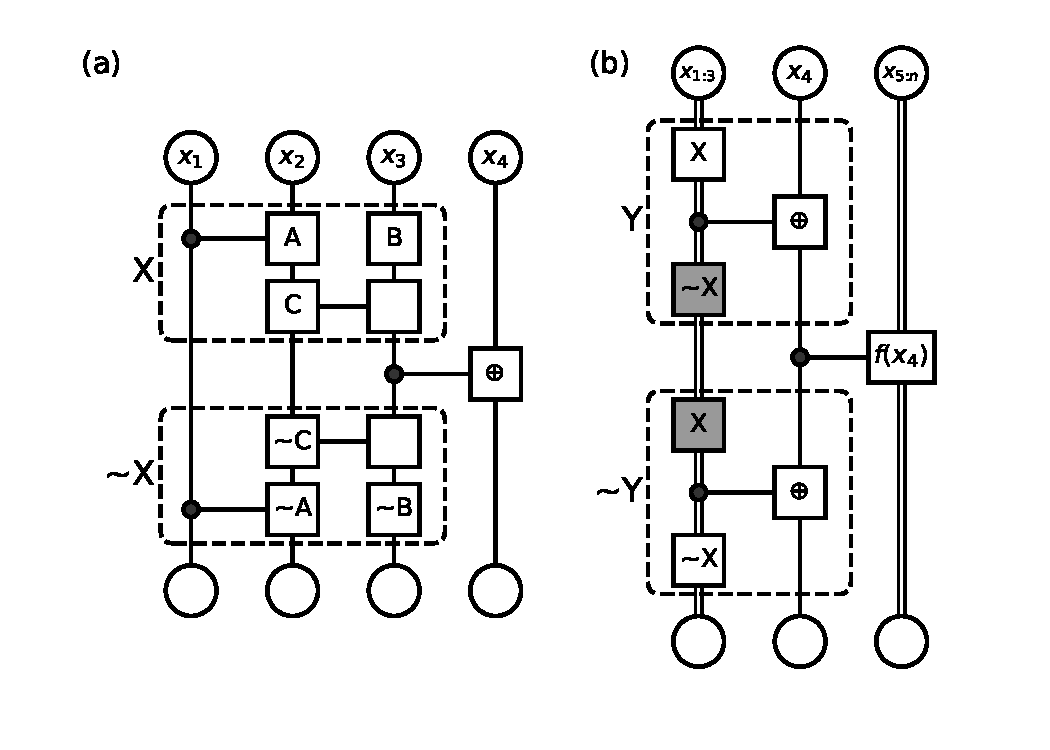
\includegraphics[width=0.6\columnwidth,trim={0 1cm 0 0cm},clip]{fig6.pdf}}
    \caption{Two computational processes represented in memory oriented computational graph, where (a) is a subprogram in (b). In these graphs, a vertical single line represents one variable, a vertical double line represents multiple variables, and a parallel line represents a function. A dot at the cross represents a control parameter of a function and a box at the cross represents a mutable parameter of a function.
    }\label{fig:ccu}
\end{figure}
To explain how it works, we introduce the memory oriented computational graph, as shown in \Fig{fig:ccu}.
Notations are highly inspired by the quantum circuit representation. A vertical line is a variable and a horizontal line is a function. When a variable is used by a function, depending on whether its value is changed or not, we put a box or a dot at the line cross. It is different from the computational graph for being a hypergraph rather than a simple graph, because a variable can be used by multiple functions now.
In panel (a). The subprogram in dashed box \texttt{X} is executed on space $x_{1\colon3}$ represents the computing stage. In the copying stage, the content in $x_3$ is read out to a pre-emptied memory $x_4$ through inplace add \texttt{+=}. Since this copy operation does not change contents of $x_{1\colon3}$, we can use the uncomputing operation \texttt{$\sim$X} to undo all the changes to these registers. Now we computing the result $x_4$ without modifying the contents in $x_{1\colon3}$. If any of them is in a known state, it can be deallocated immediately.
In panel (b), we can use the subprogram defined in (a) maked as Y to generate $x_{5\colon n}$ without modifying the contents of variables $x_{1\colon 4}$.
It is easy to see that although this uncompute-copy-uncompute design pattern can restore memories to known state, it has computational overhead.
Both $X$ and $\sim X$ are executed twice in the program (b), which is not necessary. We can cancel a pair of $X$ and $\sim X$ (the gray boxes). By doing this, we are not allowed to deallocate the memory $x_{1\colon3}$ during computing $f(x_{5\colon n})$. This is the famous time-space tradeoff that playing the central role in reversible programming.

From the lowest instruction level, whenever we reduce the symbol table (or space), the computational cost doubles.
The computational overhead grows exponentially as the uncomputating level increases, which can be seen from some of the benchmarks in the main text.
In sparse matrix multiplication and dot product, we don't introduce uncomputing in the most time consuming part, so it is $\sim0$. The space overhead is \texttt{2*m} to keep the branch decisions, which is even much smaller than the memory used to store row indices.
in Gaussian mixture model, the most time consuming matrix-vector multiplication is doubled, so it is $\sim 1$. The extra memory usage is approximately 0.5\% of the original program.
In the first kind Bessel function and bundle adjustment program, the most time consuming parts are (nestedly) uncomputed twice, hence their uncomputing level is $\sim2$.
Such aggressive uncomputing makes zero memory allocation possible.
%At last, making reversible programming an eDSL rather than an independent language allows flexible choices between reversibility and computational overhead. For example, to deallocate the memory that stores gradients in a reversible language, one has to uncompute the whole process of obtaining them.
%As an eDSL, one has an alternative to deallocate the memory irreversibly outside the scope of a reversible program, i.e., trade energy with time.

\subsection{Differentiability as a Hardware Feature}\label{sec:hardware}

\begin{figure}
    \centerline{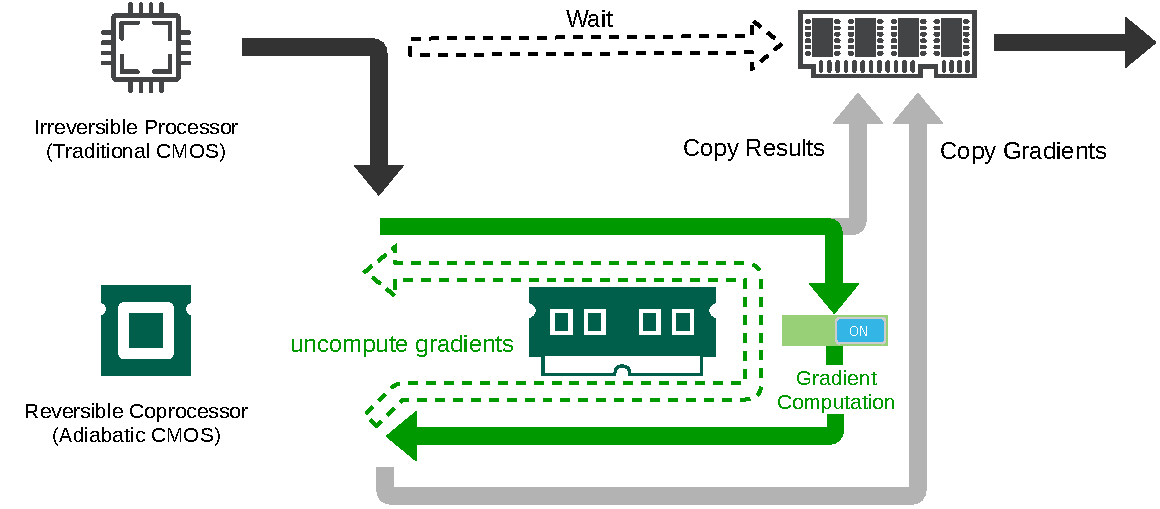
\includegraphics[width=0.8\columnwidth,trim={0 0cm 0 0cm},clip]{hardware.pdf}}
    \caption{Energy efficient AI co-processor. Green arrows represents energy efficient operations on reversible devices.}\label{fig:hardware}
\end{figure}
So far, our eDSL is compiled to Julia language. It relies on Julia's multiple dispatch to differentiate a program, which requires users to write generic programs.
A more liable AD should be a hardware or micro instruction level feature.
In the future, we can expect NiLang being compiled to reversible instructions~\cite{Vieri1999} and executed on a reversible device.
A reversible devices can play a role of differentiation engine as shown in the hetero-structural design in \Fig{fig:hardware}.
It defines a reversible instruction set and has a switch that controls whether the instruction calls a normal instruction or an instruction that also updates gradients.
When a program calls a reversible differentiable subroutine, the reversible co-processor first marches forward, compute the loss and copy the result to the main memory.
Then the co-processor execute the program backward and uncall instructions, initialize and updating gradient fields at the same time.
After reaching the starting point of the program, the gradients are transferred to the global memory.
Running AD program on a reversible device can save energy. Theoretically, the reversible routines do not necessarily cost energy, the only energy bottleneck is copying gradient and outputs to the main memory.

\subsection{The connection to Quantum programming}
A Quantum device~\cite{Nielsen2002} is a special reversible hardware that features quantum entanglement.
The instruction set of classical reversible programming is a subset of quantum instruction set.
However, building a universal quantum computer is difficult. 
Unlike a classical state, a quantum state can not be cloned. Meanwhile, it loses information by interacting with the environment.
Classical reversible computing does not enjoy the quantum advantage, nor the quantum disadvantages of non-cloning and decoherence,
but it is a model that we can try directly with our classical computer.
It is technically smooth to have a reversible computing device to bridge the gap between classical devices and universal quantum computing devices.
By introducing entanglement little by little, we can accelerate some elementary components in reversible computing. For example, quantum Fourier transformation provides an alternative to the reversible adders and multipliers by introducing the Hadamard and CPHASE quantum gates~\cite{RuizPerez2017}.
From the programming languages's perspective, most quantum programming language preassumes the existence of a classical coprocessor to control quantum devices~\cite{Svore2018}.
It is also interesting to know what is a native quantum control flow like, and does quantum entanglement provide speed up to automatic differentiation?
We believe the reversible compiling technologies will open a door to study quantum compiling.

\subsection{Gradient on ancilla problem}
In this subsection, we introduce an easily overlooked problem in our reversible AD framework.
An ancilla can sometimes carry a nonzero gradient when it is deallocated. As a result, the gradient program can be irreversible in the local scope.
In NiLang, we drop the gradient field of ancillas instead of raising an error.
In the following, we justify our decision by proving the following theorem.
\begin{theorem}
    Deallocating an ancilla with constant value field and nonzero gradient field does not introduce incorrect gradients.
\end{theorem}
\begin{proof}
    Consider a reversible function $\vx^i, b = f_i(\vx^{i-1}, a)$, where $a$ and $b$ are the input and output values of an ancilla.
    Since both $a$, $b$ are constants that are independent of input $\vx^{i-1}$, we have
\begin{align}
    \frac{\partial b}{\partial \vx^{i-1}} = \mathbf{0}.
\end{align}
Discarding gradients should not have any effect on the \texttt{value} fields of outputs.
    The key is to show $\texttt{grad(b)} \equiv \frac{\partial \vx^L}{\partial{b}}$ does appear in the \texttt{grad} fields of the output. It can be seen from the back-propagation rule 
\begin{equation}
    \frac{\partial \vx^L}{\partial \vx^{i-1}} = \frac{\partial \vx^L}{\partial \vx^i}\frac{\partial \vx^i}{\partial \vx^{i-1}} + \frac{\partial \vx^L}{\partial b}\frac{\partial b}{\partial \vx^{i-1}},
\end{equation}
where the second term with $\frac{\partial \vx^L}{\partial{b}}$ vanishes naturally. We emphasis here, the value part of discarded ancilla must be a constant.
\end{proof}

\subsection{Shared read and write problem}\label{sec:sharedrw}
One should be careful about shared read in reversible programming AD, because the shared read can introduce shared write in the adjoint program.
Let's begin with the following expression.

\begin{minipage}{.88\columnwidth}
\begin{lstlisting}
y += x * y
\end{lstlisting}
\end{minipage}

Most people will agree that this statement is not reversible and should not be allowed because it changes input variables.
We call it the \textit{simultaneous read-and-write} issue.
However, the following expression with two same inputs is a bit subtle.

\begin{minipage}{.88\columnwidth}
\begin{lstlisting}
y += x * x
\end{lstlisting}
\end{minipage}

It is reversible, but should not be allowed in an AD program because of the \textit{shared write} issue.
It can be seen directly from the expanded expression.

\begin{minipage}{.88\columnwidth}
\begin{lstlisting}
julia> macroexpand(Main, :(@instr y += x * x))
quote
    var"##253" = ((PlusEq)(*))(y, x, x)
    begin
        y = ((NiLangCore.wrap_tuple)(var"##253"))[1]
        x = ((NiLangCore.wrap_tuple)(var"##253"))[2]
        x = ((NiLangCore.wrap_tuple)(var"##253"))[3]
    end
end
\end{lstlisting}
\end{minipage}

In an AD program, the gradient field of \texttt{x} will be updated.
The later assignment to $x$ will overwrite the former one and introduce an incorrect gradient.
One can get free of this issue by avoiding using same variable in a single instruction

\begin{minipage}{.88\columnwidth}
\begin{lstlisting}
anc ← zero(x)
anc += identity(x)
y += x * anc
anc -= identity(x)
\end{lstlisting}
\end{minipage}

or equivalently,

\begin{minipage}{.88\columnwidth}
\begin{lstlisting}
y += x ^ 2
\end{lstlisting}
\end{minipage}

Share variables in an instruction can be easily identified and avoided.
However, it becomes tricky when one runs the program in a parallel way.
For example, in CUDA programming, every thread may write to the same gradient field of a shared scalar.
How to solve the shared write in CUDA programming is still an open problem, which limits the power of reversible programming AD on GPU.



\subsection{Several future directions}\label{sec:outlook}

We can use NiLang to solve some existing issues related to AD.
We can use it to generate AD rules for existing machine learning packages like \href{https://github.com/JuliaDiff/ReverseDiff.jl}{ReverseDiff}, Zygote~\cite{Innes2019}, Knet~\cite{Yuret2016}, and Flux~\cite{Innes2018a}.
Many backward rules for sparse arrays and linear algebra operations have not been defined yet in these packages.
We can also use the flexible time-space tradeoff in reversible programming to overcome the memory wall problem in some applications.
A successful, related example is the memory-efficient domain-specific AD engine in quantum simulator Yao~\cite{Luo2019}.
This domain-specific AD engine is written in a reversible style and solved the memory bottleneck in variational quantum simulations. It also gives so far the best performance in differentiating quantum circuit parameters.
Similarly, we can write memory-efficient normalizing flow~\cite{Kobyzev2019} in a reversible style. Normalizing flow is a successful class of generative models in both computer vision~\cite{Kingma2018} and quantum physics~\cite{Dinh2016,Li2018}, where its building block bijector is reversible.
We can use a similar idea to differentiate reversible integrators~\cite{Hut1995, Laikov2018}.
With reversible integrators, it should be possible to rewrite the control system in robotics~\cite{Giftthaler2017} in a reversible style, where scalar is a first-class citizen rather than tensor.
Writing a reversible control program should boost training performance.
Reversibility is also a valuable resource for training.

To solve the above problems better, reversible programming should be improved from multiple perspectives.
First, we need a better compiler for compiling reversible programs.
To be specific, a compiler that admits mutability of data, and handle shared read and write better.
Then, we need a reversible number system and instruction set to avoid rounding errors and support reversible control flows better.
There are proposals of reversible floating point adders and multipliers, however these designs require allocating garbage bits in each operation~\cite{Nachtigal2010,Nachtigal2011,Nguyen2013,Hner2018}.
In NiLang, one can simulate rigorous reversible arithmetic with the fixed-point number package \href{https://github.com/JuliaMath/FixedPointNumbers.jl}{FixedPointNumbers}.
However, a more efficient reversible design requires instruction-level support.
Some other numbers systems are reversible under \texttt{*=} and \texttt{/=} rather than \texttt{+=} and \texttt{-=}, including \href{https://github.com/cjdoris/LogarithmicNumbers.jl}{LogarithmicNumbers}~\cite{Taylor1988} and \href{https://github.com/GiggleLiu/TropicalNumbers.jl}{TropicalNumbers}.
They are powerful tools to solve domain specific problems, for example, we have an upcoming work about differentiating over tropical numbers to solve the ground state configurations of a spinglass system efficiently.
We also need \texttt{comefrom} like instruction as a partner of \texttt{goto} to specify the postconditions in our instruction set.
Finally, although we introduced that the adiabatic CMOS as a better choice as the computing device in a spacecraft~\cite{Debenedictis2017}.
There are some challenges in the hardware side too, one can find a proper summary of these challenges in \Ref{Frank2005b}.

Solutions to these issues requires the participation of people from multiple fields.

\bibliographystyle{apsrev4-1}
\bibliography{invc}

\end{document}
